% ============================================================
%  Figure captions for:
%  Partition-State Graph Search for Tandem Mass Spectrometry
% ============================================================

\begin{figure*}[!htbp]
    \centering
    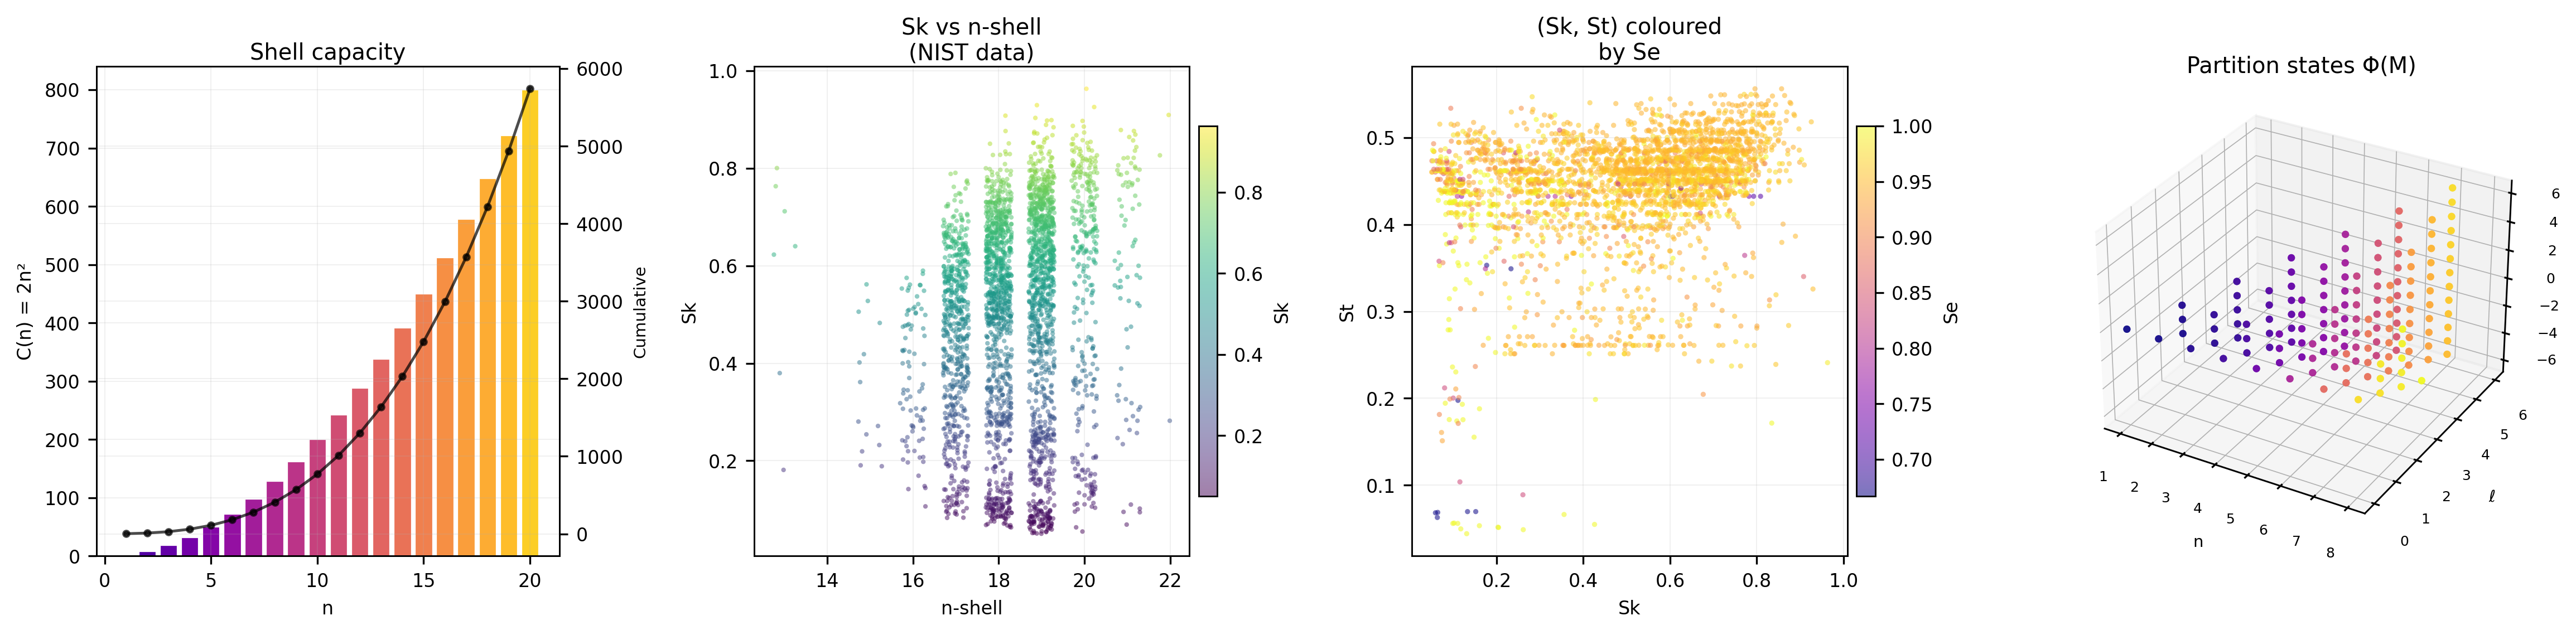
\includegraphics[width=\textwidth]{figures/panel_01_bijection_embedding.png}
    \caption{\textbf{The partition bijection and its S-entropy embedding: discrete partition states map into a continuous metric space suitable for graph search.}
    (\textbf{A}) Shell capacity $C(n)=2n^2$ (bars, plasma scale) with the cumulative count $N_{\mathrm{state}}(n)=n(n+1)(2n+1)/3$ overlaid on a twin axis (black markers). The quadratic per-shell capacity and cubic cumulative growth together define the size of the node set $\mathcal{V}=\Parts$ available to the search graph.
    (\textbf{B}) Scatter of the knowledge-entropy coordinate $S_k$ versus precursor $n$-shell for the 3{,}000 NIST AC\_CAC spectra (jittered horizontally, coloured by $S_k$). The near-linear envelope confirms the embedding $S_k=(n-1)/(n_P-1)$: principal level maps monotonically to the kinetic-entropy axis.
    (\textbf{C}) Scatter of $(S_k,S_t)$ for all spectra, coloured by the evolution-entropy coordinate $S_e$. The points populate a broad region of the $S_k$--$S_t$ plane with $S_e$ concentrated near unity (harmonic-dense fragment spectra), visualising the three-dimensional structure that distinguishes isobaric ions sharing an $m/z$ but differing in structural entropy.
    (\textbf{D}) Three-dimensional scatter of the first $300$ partition states in $(n,\ell,m)$ coordinates, coloured by bijection index $M$ on the plasma scale. The triangular-prism filling ($0\le\ell<n$, $|m|\le\ell$) and the monotone colour gradient confirm that $\PhiMap:\Zp\to\Parts$ assigns each integer to exactly one node, providing the canonical identity for every ion in the graph.}
    \label{fig:sg-1}
\end{figure*}

\begin{figure*}[!htbp]
    \centering
    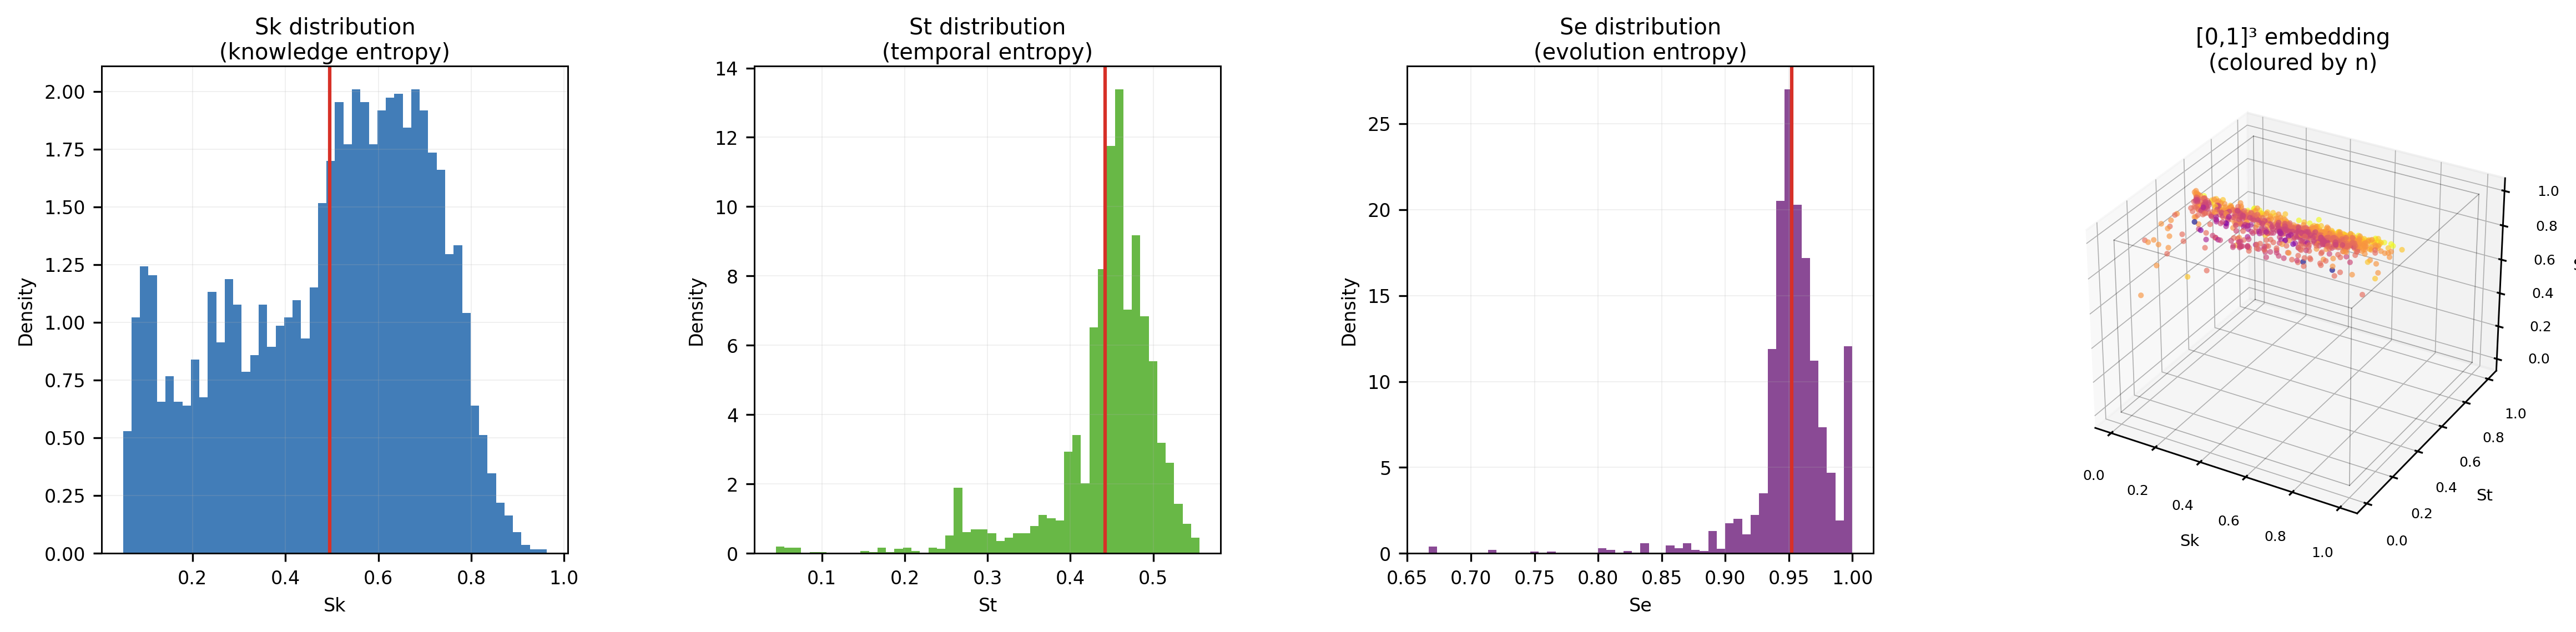
\includegraphics[width=\textwidth]{figures/panel_02_sentropy_distributions.png}
    \caption{\textbf{S-entropy coordinate distributions over 3{,}000 NIST spectra: all ions occupy the unit cube $[0,1]^3$ (Proposition: coordinate validity $=1.000$).}
    (\textbf{A}) Density histogram of the knowledge entropy $S_k$ (Shannon entropy of the normalised fragment-intensity distribution), with the mean marked (red). The broad distribution (mean $\approx 0.50$, standard deviation $\approx 0.21$) shows that the library spans the full kinetic-entropy axis.
    (\textbf{B}) Density histogram of the temporal entropy $S_t$ (logarithmic span of the fragment $m/z$ range), concentrated around $0.44$ with a narrow spread, reflecting the characteristic mass-range ratio of amino acid and acylcarnitine fragments.
    (\textbf{C}) Density histogram of the evolution entropy $S_e$ (fraction of harmonically proximate fragment pairs), concentrated near $0.95$, indicating that fragment $m/z$ ratios are dominated by near-rational relationships---the spectral signature of a common partition origin.
    (\textbf{D}) Three-dimensional scatter of all spectra in the $(S_k,S_t,S_e)$ unit cube (wireframe shown), coloured by precursor $n$-shell on the plasma scale. Every point lies strictly inside the cube, providing direct visual confirmation that the S-entropy embedding maps all $3{,}000$ empirical ions into the bounded metric space on which Dijkstra search operates.}
    \label{fig:sg-2}
\end{figure*}

\begin{figure*}[!htbp]
    \centering
    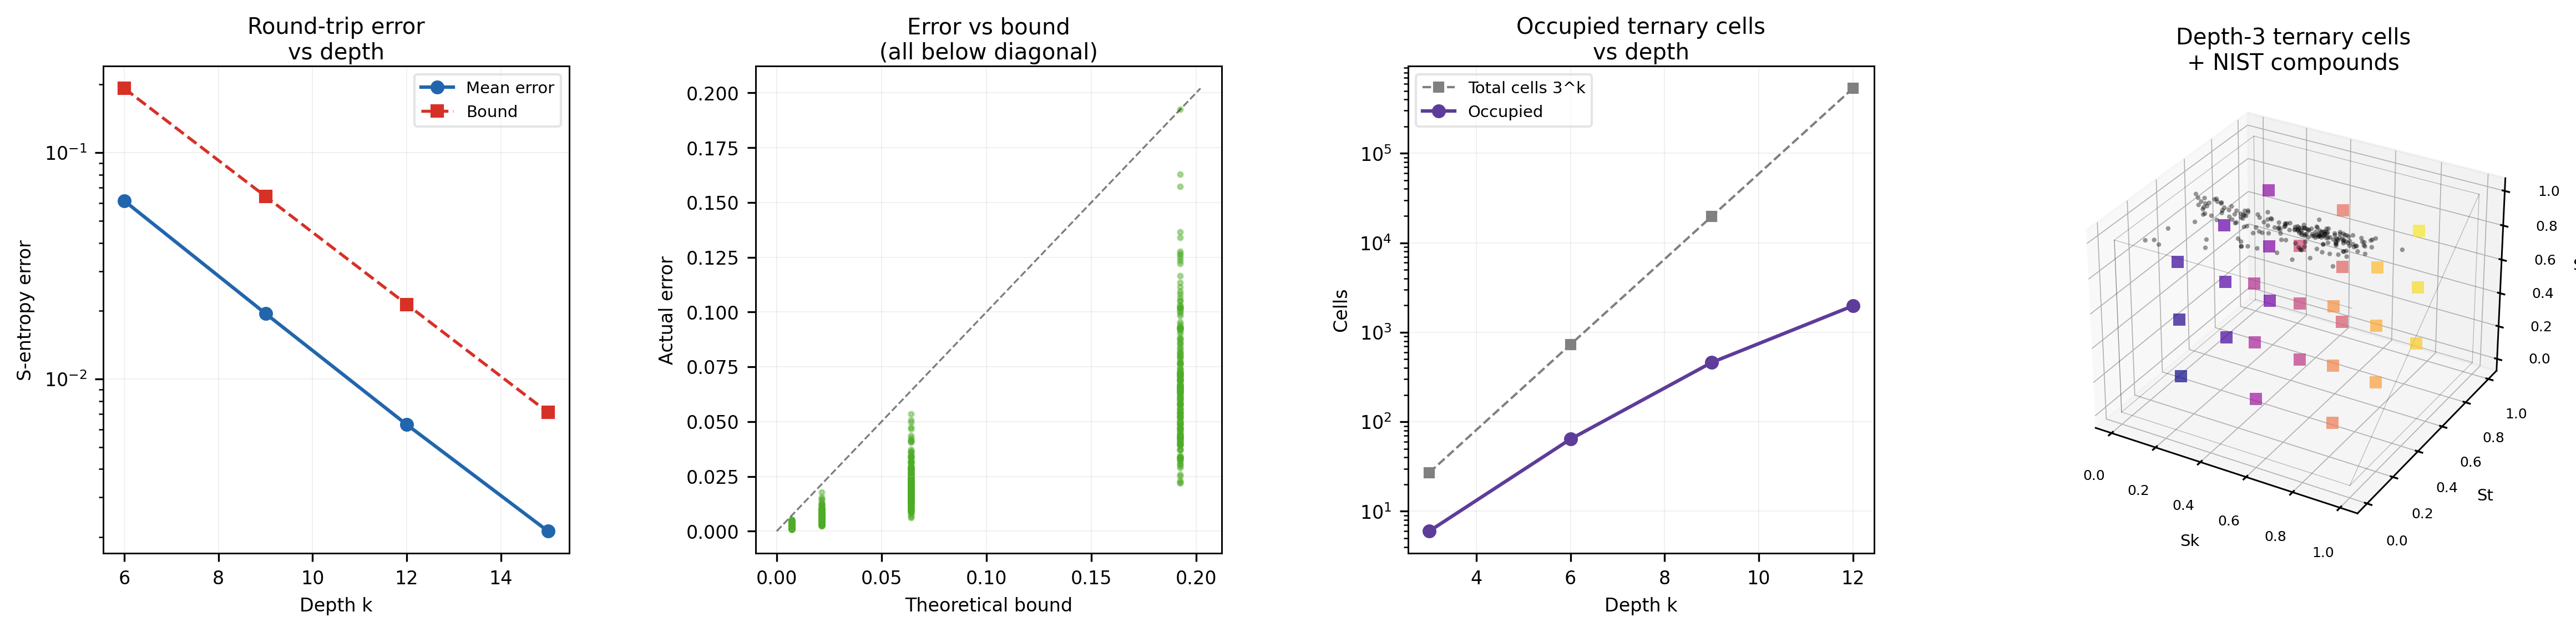
\includegraphics[width=\textwidth]{figures/panel_03_ternary_encoding.png}
    \caption{\textbf{Interleaved ternary encoding: round-trip error stays below the distance bound $\sqrt{3}\cdot 3^{-\lfloor k/3\rfloor}$ at every depth.}
    (\textbf{A}) Mean encode--decode round-trip error (blue circles) and the theoretical bound $\sqrt{3}\cdot 3^{-\lfloor k/3\rfloor}$ (red dashed squares) versus encoding depth $k\in\{6,9,12,15\}$ on a logarithmic axis. The mean error lies strictly below the bound at every depth and decreases geometrically, confirming the distance-preservation theorem.
    (\textbf{B}) Scatter of actual round-trip error versus theoretical bound across all depths and a 200-spectrum sample, with the identity line (black dashed). Every point lies below the diagonal, confirming that the ternary cell containing a state always lies within the predicted radius of the state itself.
    (\textbf{C}) Number of occupied ternary cells (purple circles) versus total available cells $3^k$ (grey squares) as a function of depth on a logarithmic axis. The occupied count rises toward full uniqueness as depth increases, while remaining far below the exponentially growing total---the basis for the sparse, lazily-materialised dictionary.
    (\textbf{D}) Three-dimensional view of the $27$ depth-3 ternary cell centres (coloured squares) within the $(S_k,S_t,S_e)$ unit cube, overlaid with NIST compound positions (black points). The compounds cluster into a subset of the available cells, demonstrating that ternary addressing groups spectrally similar molecules by common prefix without any chemical knowledge being encoded.}
    \label{fig:sg-3}
\end{figure*}

\begin{figure*}[!htbp]
    \centering
    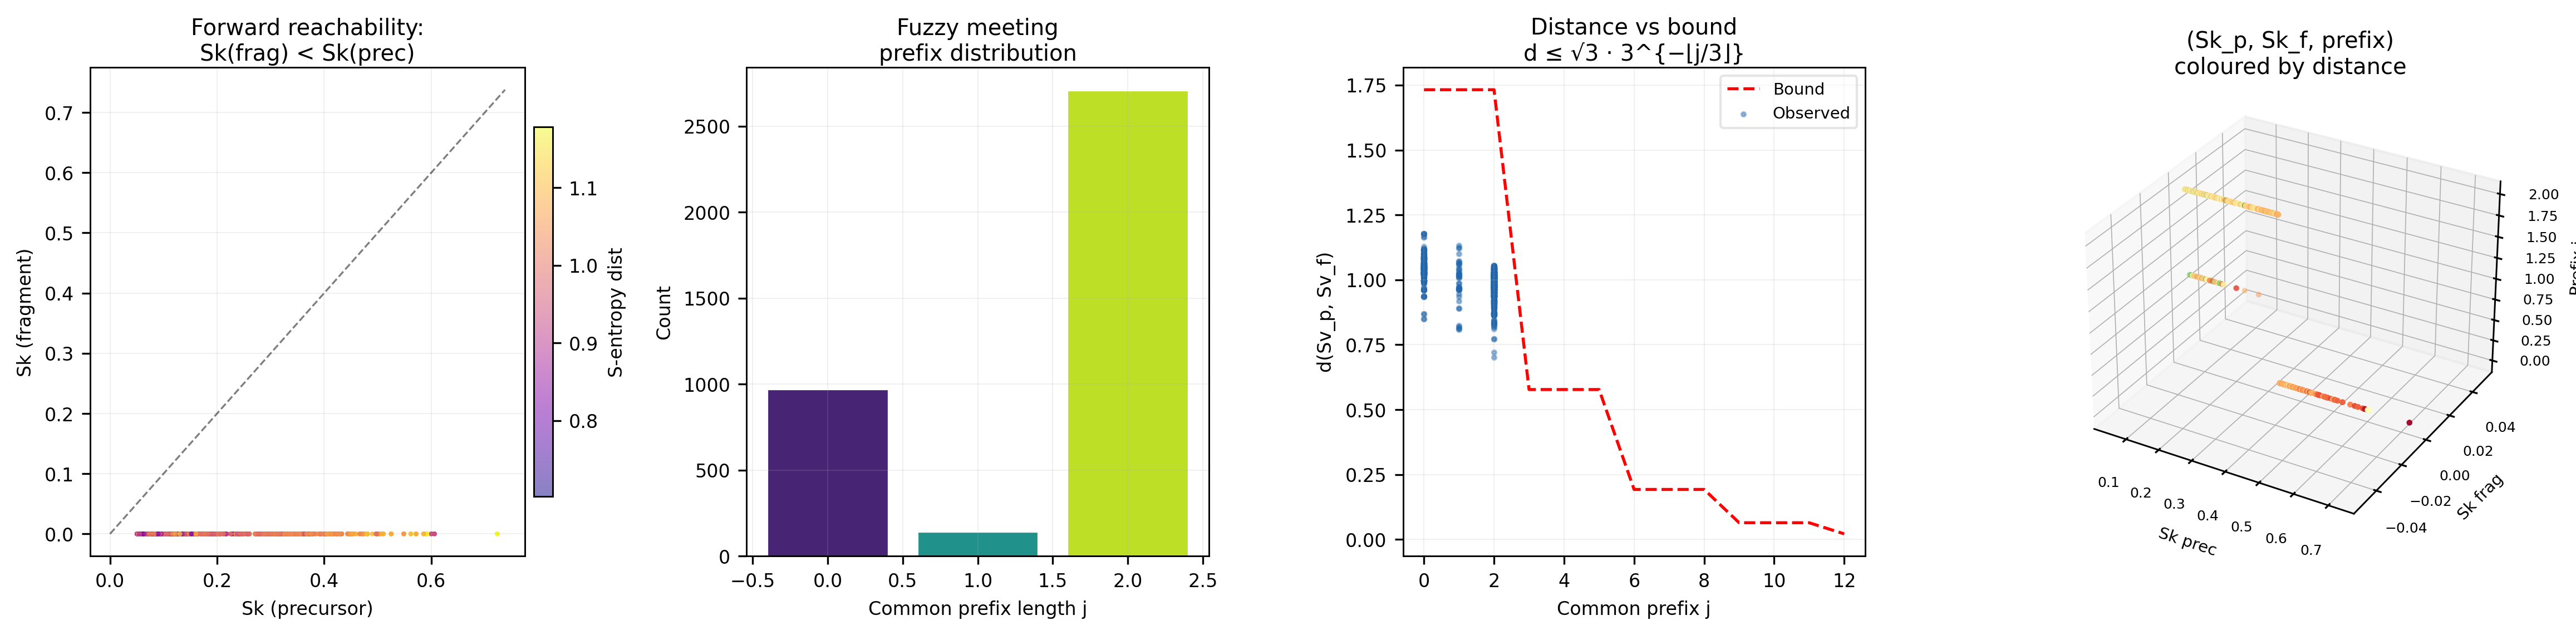
\includegraphics[width=\textwidth]{figures/panel_04_sebd_search.png}
    \caption{\textbf{SEBD-MS bidirectional search: every fragment is forward-reachable ($S_k$ ordering $=1.000$) and the fuzzy meeting condition respects the distance bound.}
    (\textbf{A}) Scatter of fragment $S_k$ versus precursor $S_k$ for all pairs, coloured by S-entropy distance, with the identity line (black dashed). Every point lies below the diagonal ($S_k^{\mathrm{frag}}<S_k^{\mathrm{prec}}$), confirming that all observed fragments lie in the forward reachability cone and that the physical fragment graph is a directed acyclic graph.
    (\textbf{B}) Distribution of the common-prefix length $j$ at which precursor and fragment ternary addresses agree (bars, viridis scale). The distribution is concentrated at small $j$ (mean $\approx 0.24$), showing that precursor and fragment occupy widely separated regions of S-entropy space and that the bidirectional frontiers meet at coarse resolution---the source of the search-space reduction.
    (\textbf{C}) S-entropy distance $d(\mathbf{S}_p,\mathbf{S}_f)$ versus common prefix $j$ (blue points) overlaid with the bound $\sqrt{3}\cdot 3^{-\lfloor j/3\rfloor}$ (red dashed). All observed distances fall below the bound, confirming the fuzzy-meeting-radius theorem that links prefix agreement to metric proximity.
    (\textbf{D}) Three-dimensional scatter of precursor--fragment pairs in $(S_k^{\mathrm{prec}},S_k^{\mathrm{frag}},\text{prefix})$ space, coloured by S-entropy distance on a reversed red--green scale. The structure shows that pairs sharing longer prefixes (higher on the prefix axis) have smaller distances (greener), the geometric basis for the bidirectional meeting-point optimisation.}
    \label{fig:sg-4}
\end{figure*}

\begin{figure*}[!htbp]
    \centering
    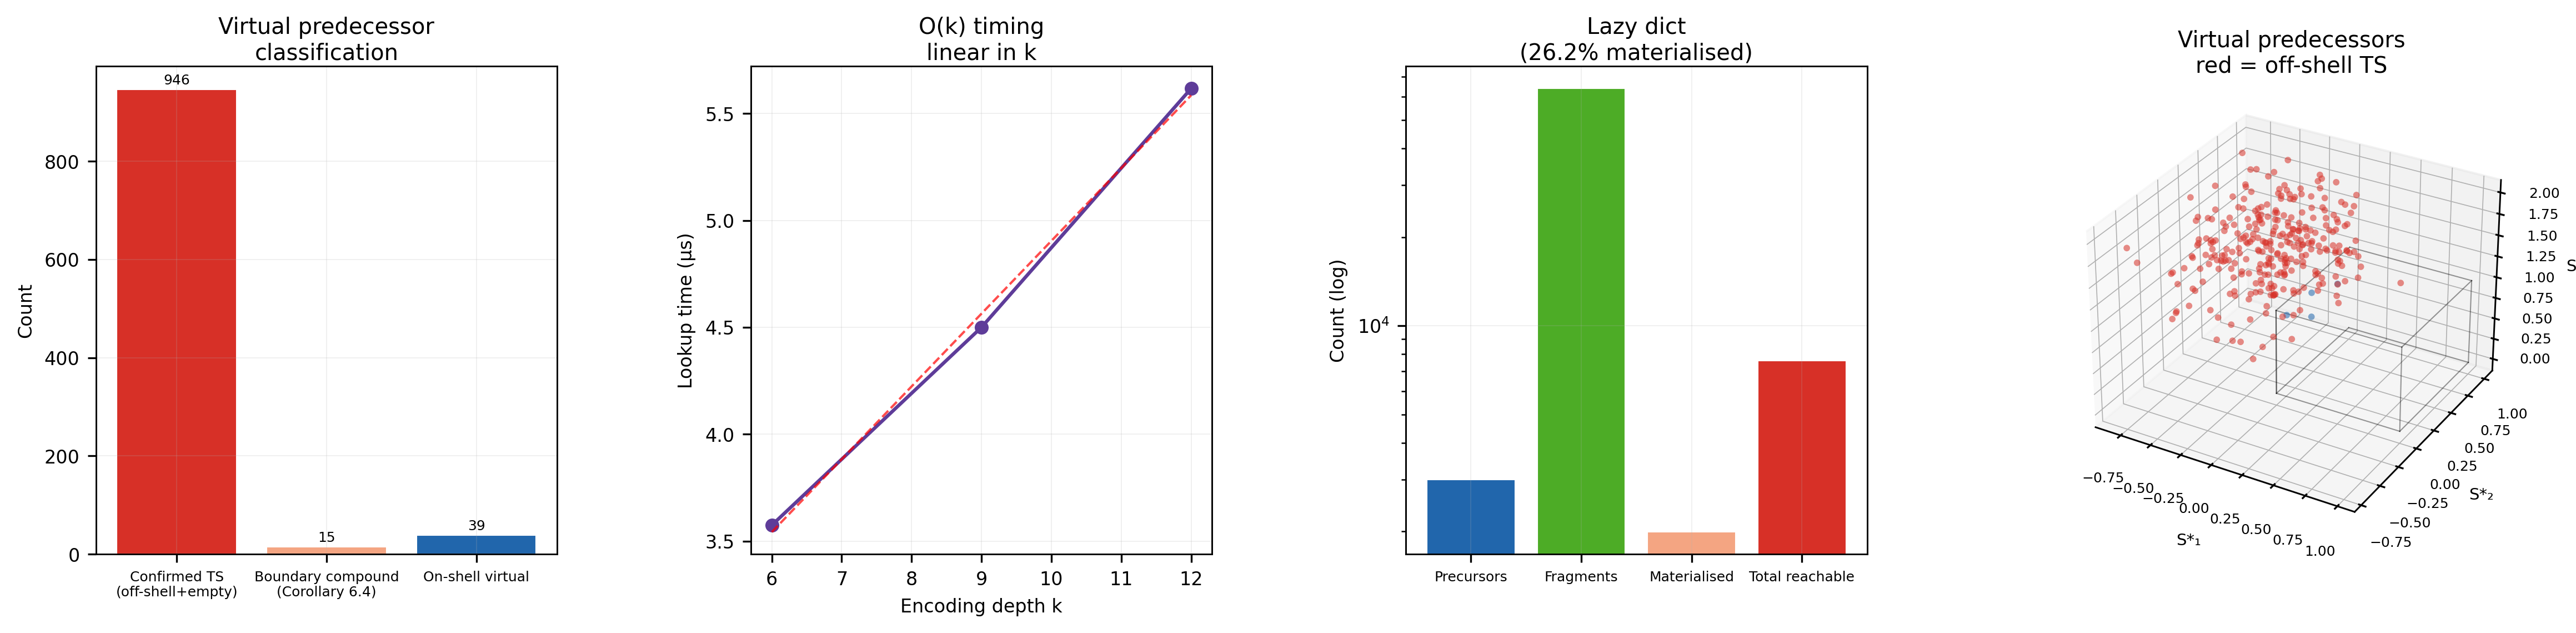
\includegraphics[width=\textwidth]{figures/panel_05_virtual_lazy.png}
    \caption{\textbf{Virtual substates and the lazy dictionary: off-shell predecessors are detected by empty lookup, and only $26\%$ of reachable states are ever materialised.}
    (\textbf{A}) Classification of virtual predecessors $\mathbf{S}^{*}=2\mathbf{S}_f-\mathbf{S}_2$: confirmed transition states (off-shell with empty lookup, red), boundary compounds (off-shell with non-empty lookup, orange; Corollary on database-driven discovery), and on-shell virtual components (blue). The dominance of the red bar confirms that off-shell predecessors are correctly identified as transition states by the empty-lookup test alone.
    (\textbf{B}) Lookup time (\textmu s) versus encoding depth $k$ for the largest trie (purple circles) with a linear fit (red dashed). The positive linear trend confirms the $\mathcal{O}(k)$ search complexity: lookup time grows with encoding depth, not with database size.
    (\textbf{C}) Counts of precursors, fragments, materialised dictionary entries, and total reachable partition states on a logarithmic axis. The materialised count ($26.2\%$ of reachable states) sits far below the total, confirming that the lazy dictionary stores only visited nodes---a four-fold memory saving here, growing to orders of magnitude for large molecules.
    (\textbf{D}) Three-dimensional scatter of virtual predecessor coordinates $\mathbf{S}^{*}$ within the unit-cube wireframe: on-shell components inside the cube (blue) and off-shell transition states outside it (red). The off-shell points, lying beyond $[0,1]^3$, are exactly those returning empty trie lookups, providing visual confirmation that emptiness of the lazy dictionary characterises the transition states of the fragmentation pathway.}
    \label{fig:sg-5}
\end{figure*}
